\section{Background: Goal-oriented Requirements Language and argument schemes}
\label{sect:background}

In this section, we first introduce our running example, after which we introduce the Goal-oriented Requirements Language (GRL)~\cite{Amyot:2010:EGM:1841349.1841356}, which is the goal modeling language we use to integrate with the argumentation framework. Lastly, we introduce argument schemes, and in particular, we discuss the \emph{practical reasoning argument scheme (PRAS)}~\cite{atkinson2007}, which is an argument scheme that is used to form arguments and counter-arguments about situations involving goals. This will be our starting point in the next section.

\subsection{Running example: Traffic Simulator}
\label{sect:goals:runningexample}

Most of the examples in this article, as well as the topic of discussion in the transcripts we analyze, come from the traffic simulator design exercise. In this exercise, designers are provided a problem description, requirements, and a description of the desired outcomes. The problem description is given in full in Appendix~\ref{ch:designprompt}, and is summarized as follows: The client of the project is Professor E, who teaches civil engineering at UCI. It is the task of the designer to specify a system in which the professor can teach students how various theories around traffic lights works, such as queuing theory. To this end, a piece of software has to be developed in which students can create visual maps of an area, regulate traffic, and so forth. The original version of the problem descrption~\cite{UCIworkshop} is well known in the field of design reasoning since it has been used in a workshop\footnote{\url{http://www.ics.uci.edu/design-workshop/}}, and transcripts of this workshop have been analyzed in detail~\cite{Petre:2013:SDA:2535028}. Although the concepts of traffic lights, lanes, and intersections are common and appear to be simple, building a traffic simulator to represent these relationships and events in real time turns out to be challenging.

\subsection{Goal-oriented Requirements Language (GRL)}
\label{sect:background:grl}
GRL is a visual modeling language for specifying intentions, business goals, and \emph{non-functional requirements} of multiple stakeholders \cite{Amyot:2010:EGM:1841349.1841356}. GRL is part of the User Requirements Notation, an ITU-T standard, that combines goals and non-functional requirements with functional and operational requirements (i.e. use case maps) in one. GRL can be used to specify alternatives that have to be considered, decisions that have been made, and rationales for making decisions. A GRL model is a connected graph of intentional elements that optionally are part of actors. All the elements and relationships used in GRL are shown in Figure~\ref{fig:grl_legend}.

\begin{figure*}[ht]
\centering
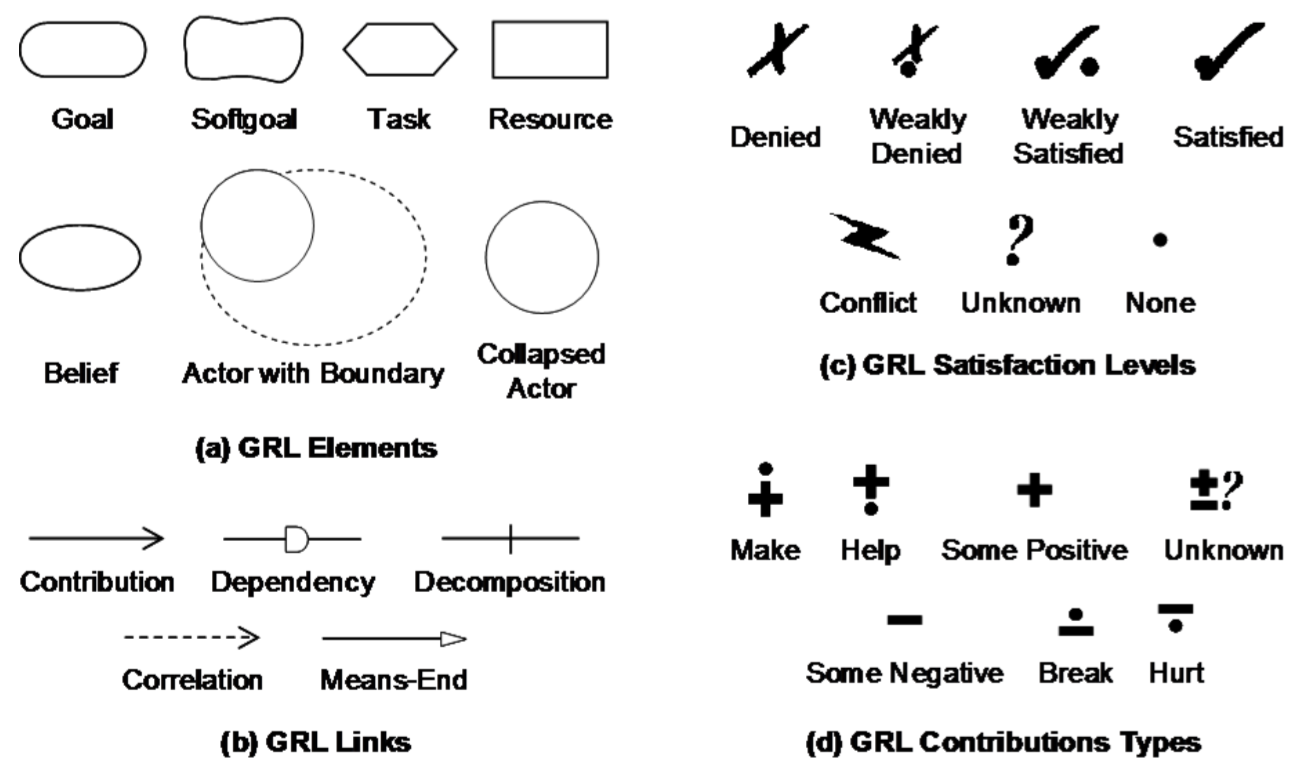
\includegraphics[scale=0.6]{img/grl_legend}
\caption{Basic elements and relationships of GRL}
\label{fig:grl_legend}
\end{figure*}

Figure~\ref{fig:trafficsim} illustrates a GRL diagram from the traffic simulator design exercise. An actor (
\includegraphics[scale=1]{img/actor}) represents a stakeholder of a system (\texttt{Student}, Figure~\ref{fig:trafficsim}), or the system itself ( \texttt{Traffic Tycoon}, Figure~\ref{fig:trafficsim}). Actors are holders of intentions; they are the active entities in the system or its environment who want goals to be achieved, tasks to be performed, resources to be available, and softgoals to be satisfied. Softgoals (
\includegraphics[scale=1]{img/softgoal}) differentiate themselves from goals (
\includegraphics[scale=1]{img/goal}) in that there is no clear, objective measure of satisfaction for a softgoal whereas a goal is quantifiable, often in a binary way. Softgoals (e.g.  \texttt{Realistic simulation)} are often more related to non-functional requirements, whereas goals (such as  \texttt{Generate cars}) are more related to functional requirements. Tasks (
\includegraphics[scale=1]{img/task}) represent solutions to (or operationalizations of) goals and softgoals. In Figure~\ref{fig:trafficsim}, some of the tasks are  \texttt{Create new cars} and \texttt{Keep same cars}. In order to be achieved or completed, softgoals, goals, and tasks may require resources (
\includegraphics[scale=1]{img/resource}) to be available (e.g., \texttt{External Library}, Figure~\ref{fig:trafficsim}).

\begin{figure*}[ht]
\centering
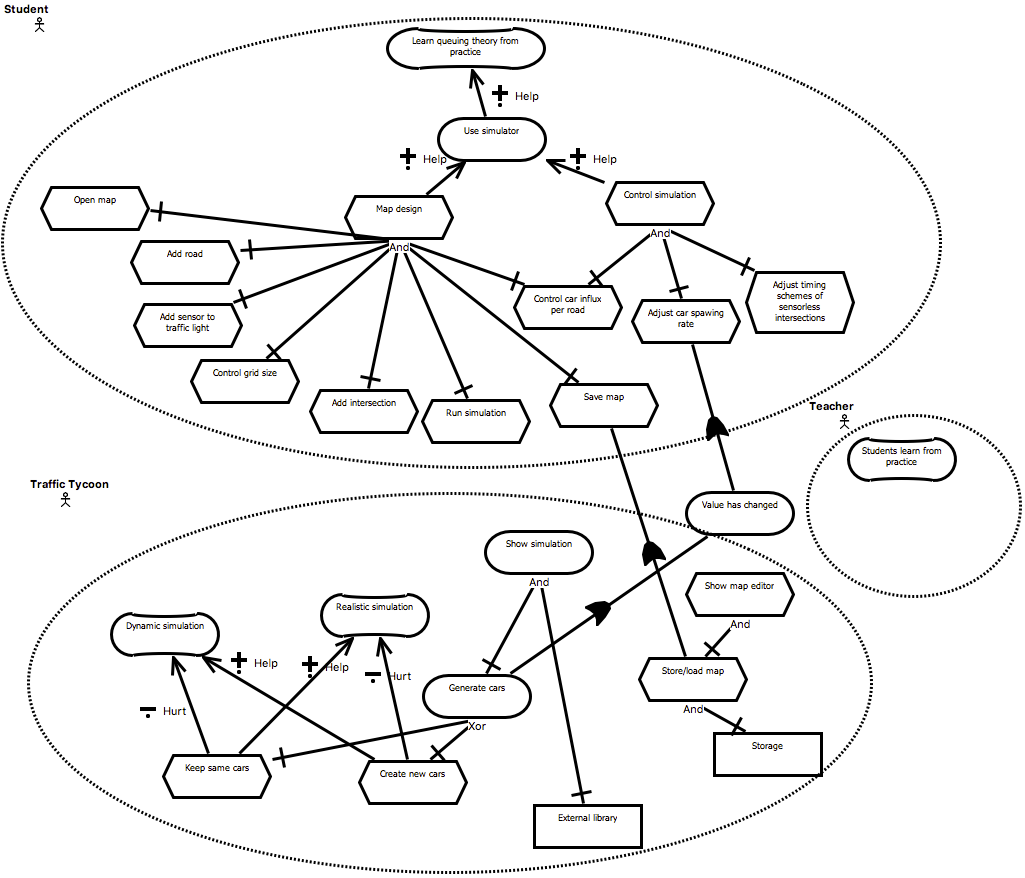
\includegraphics[width=\textwidth]{img/transcript_grl_0}
\caption{GRL Model for the traffic simulator.}
\label{fig:trafficsim}
\end{figure*}

Different links connect the elements in a GRL model. AND, IOR, and XOR decomposition links (
\includegraphics[scale=1]{img/decomposition}) allow an element to be decomposed into sub-elements. In Figure~\ref{fig:trafficsim}, the goal  \texttt{Generate cars} is XOR-decomposed to the tasks \texttt{Create new cars} and \texttt{Keep same cars}. Contribution links (
\includegraphics[scale=1]{img/contribution}) indicate desired impacts of one element on another element. A contribution link has a qualitative contribution type or a quantitative contribution. Task  \texttt{Create new cars} has a \emph{help} qualitative contribution to the softgoal  \texttt{Dynamic simulation}. Dependency links (
\includegraphics[scale=1]{img/dependency}) model relationships between actors. For example, actor  \texttt{Traffic Tycoon} depends on the actor  \texttt{Student} to perform the task  \texttt{Adjust car spawning rate} to fulfill its task  \texttt{Generate cars}.

GRL is based on $i*$~\cite{Yu:1997:TMR:827255.827807} and the NFR Framework~\cite{chung2012non}, but it is not as restrictive as $i*$. Intentional elements and links can be more freely combined, the notion of agents is replaced with the more general notion of actors, i.e., stakeholders, and a task does not necessarily have to be an activity performed by an actor, but may also describe properties of a solution. GRL has a well-defined syntax and semantics, which are necessary if we want to incorporate it into a formal framework (requirements 1 and 2 as described in the introduction). Furthermore, GRL provides support for providing a scalable and consistent representation of multiple views/diagrams of the same goal model (see~\cite[Ch.2]{Ghanavati2013} for more details). GRL is also linked to Use Case Maps via URNLink ((
\includegraphics[scale=1]{img/urnlink}) which provides traceability between concepts and instances of the goal model and behavioral design models. Multiple views and traceability are a good fit with our current research: we aim to add traceability links between intentional elements and their underlying arguments. 

GRL has six evaluation algorithms which are semi-automated and allow the analysis of alternatives and design decisions by calculating the satisfaction value of the intentional elements across multiple diagrams quantitatively, qualitatively or in a hybrid way. The satisfaction values from intentional elements in GRL can also be propagated to use case maps elements.  jUCMNav, GRL tool-support, also allows for adding new GRL evaluation algorithms~\cite{jUCMNav}. GRL also has the capability to be extended through metadata, links, and external OCL constraints. This allows GRL to be used in many domains without the need to change the whole modeling language. This feature also helps us to apply our argumentation to other domain such as compliance, which we explain in more detail in Section~\ref{sect:goalmodeling:openissues}.

The GRL model in Figure~\ref{fig:trafficsim} shows the softgoals, goals, tasks and the relationship between the different intentional elements in the model. However, the rationales and arguments behind certain intentional elements are not shown in the GRL model. Some of the questions that might be interesting to know about are the following:

\begin{itemize}
	\item Why does actor \texttt{Teacher} have only a single softgoal \texttt{Students learn from practice}? Why is this, for instance, not connected to any of the elements of \texttt{Student}?
	\item What does  \texttt{Adjust timing schemes of sensorless interactions} mean?
	\item Why does task \texttt{Keep same cars} contribut positively to \texttt{Realistic simulation} and negatively to \texttt{Dynamic simulation}?
	\item How does the \texttt{Student} control the \texttt{Traffic Tycoon}?
	\item Why does \texttt{Map design} have so many decompositions into other tasks?
\end{itemize}

These are the type of the questions that we cannot answer just by looking at the GRL models. The model in Figure~\ref{fig:trafficsim} does not contain information about discussions that let up to the resulting elements of the model, such as various clarification steps for the naming, or alternatives that have been considered for the relationships. In this article we aim to address this shortcoming.

\subsection{Argument Scheme for Practical Reasoning (PRAS)}
\label{sect:background:pras}

Reasoning about which goals to pursue and actions to take is often referred to as \emph{practical reasoning}, and has been studied extensively in philosophy (e.g. \cite{Raz1978-RAZPR,walton1990}) and artificial intelligence \cite{bratman1987,atkinson2007}. One approach is to capture practical reasoning in terms of arguments schemes and critical questions~\cite{walton1990}. The idea is that an instantiation of such a scheme gives a presumptive argument in favor of, for example, taking an action. This argument can, then, be tested by posing critical questions about, for instance, whether the action is possible given the situation, and a negative answer to such a question leads to a counterargument to the original presumptive argument for the action. 

A formal approach to persuasive and deliberative reasoning about goals and actions has been presented by Atkinson et al.~\cite{atkinson2007}, who define the \emph{practical reasoning argument scheme} (PRAS). PRAS follows the following basic argument structure. 

\begin{itemize}
\item[] We have goal $G$,
\item[] Doing action $A$ will realize goal $G$,
\item[] Which will promote the value $V$
\item[] \textit{Therefore} 
\item[] We should perform action $A$
\end{itemize}

So, for example, we can say that 
\begin{itemize}
\item[] We have goal  \texttt{Generate traffic},
\item[]  \texttt{Keep same cars} will realize goal  \texttt{Generate traffic},
\item[] Which will promote the value  \texttt{Simple design}
\item[] \textit{Therefore} 
\item[] We should perform action  \texttt{Keep same cars}
\end{itemize}

Practical reasoning is defeasible, in that conclusions which are at one point acceptable can later be rejected because of new information. Atkinson \emph{et al.}~\cite{atkinson2007} define a set of critical questions that point to typical ways in which a practical argument can be criticized by, for example, questioning the validity of the elements in the scheme or the connections between the elements. Some examples of critical questions are as follows.

\begin{enumerate}
\item Will the action bring about the desired goal?
%\item Does the goal promote the value stated?
\item Are there alternative ways of realizing the same goal?
\item Are there alternative ways of promoting the same value?
%\item Does doing the action have a side effect which demotes the value?
\item Does doing the action have a side effect which demotes some other value?
\item Does doing the action promote some other value?
%\item Does doing the action preclude some other action which would promote some other value?
\item Is the action possible?
\item Can the desired goal be realized?
\item Is the value indeed a legitimate value?
\end{enumerate}

These critical questions can point to new arguments that might counter the original argument. Take, for example, critical question 4: if we find that  \texttt{Keep same cars} actually negatively influences the value  \texttt{Realistic simulation}, we have a counterargument to the above argument. Another way to counter an argument for an action is to suggest an alternative action that realizes the same goal (question 2) or an alternative goal that promotes the same value (question 3). For example, we can argue that  \texttt{Create new cars} also realizes the goal  \texttt{Generate traffic}, which gives us a counterargument to the original argument -- to generate traffic by simply keeping the cars that disappear off the screen and have them wrap around to the other side of the screen -- that also follows PRAS.

In argumentation, counterarguments are said to \emph{attack} the original arguments (and sometimes vice versa). In the work of Atkinson et al.~\cite{atkinson2007}, arguments and their attacks are captured as an \emph{argumentation framework} of arguments and attack relations as introduced by Dung~\cite{Dung1995}\footnote{Full definitions of Dung's~\cite{Dung1995} frameworks and semantics will be given in section \ref{sect:gmas}. In this section, we will briefly discuss the intuitions behind these semantics.}. Figure \ref{fig:pras:example} shows an argumentation framework with three arguments from the above example: the argument for  \texttt{Keep same cars} (A1), the argument for \texttt{Create new cars} (A3), and the argument that \texttt{Keep same cars} demotes the value  \texttt{Realistic simulation} (A2). The two alternative PRAS instantiations are A1 and A3. These arguments mutually attack each other, as \texttt{Keep same cars}  and \texttt{Create new cars} are considered to be mutually exclusive. Argument A2 attacks A1, as it points to a negative side-effect of \texttt{Keep same cars}. 

\begin{figure}[ht!]
\centering
\begin{tikzpicture}
        \node[minimum size=1cm] (att3) [argNodeIN] at (0,-3) {$A_3$};
        \node[minimum size=1cm] (att1) [argNodeOUT] at (0,0) {$A_1$};
        \node[minimum size=1cm] (att2) [argNodeIN] at (3,0) {$A_2$};
         \path
    (att2) edge [attackLink] (att1)
    (att1) edge [attackLink,<->] (att3);
\end{tikzpicture}
\caption{Example argumentation framework.}
\label{fig:pras:example}
\end{figure}

Given an argumentation framework, the acceptability of arguments can be determined according to the appropriate argumentation semantics. The intuition is that an argument is acceptable if it is \emph{undefeated}, that is, any argument that attacks it, is itself defeated. In the argumentation framework in Figure~\ref{fig:pras:example}, argument A2 is undefeated because it has no attackers. This makes A1 defeated, because one of its attackers, A2, is undefeated. A3 is then also undefeated, since its only attacker, A1, is defeated by A2. Thus, the set of undefeated (justified) arguments given the argumentation framework in Figure~\ref{fig:pras:example} is $\{$A2, A3$\}$, corresponding to arguments for \texttt{Realistic simulation} and \texttt{Create new cars}.

\subsubsection*{Practical Argumentation and Goal Modeling}
\label{sect:background:pras:motivation}

Practical reasoning in the PRAS framework as described above provides a formal framework for defeasible reasoning about goals and actions that adheres to the acceptability semantics of Dung~\cite{Dung1995} and its various extensions \cite{amgoud2002reasoning,modgil2009}. The usefulness of PRAS for the analysis of practical reasoning situations has been shown in different areas such as e-democracy~\cite{cartwright2009IS}, law~\cite{atkinson2005legal}, planning \cite{medellin2013planning} and choosing between safety critical actions \cite{tolchinsky2012deliberation}. In this article, we aim at capturing the stakeholder's discussions as formal argumentation based on PRAS to decide whether intentional elements and their relationships are shown in the resulting goal model. This give a rationalization to the elements of the goal model in terms of underlying arguments, and furthermore, it allows one to understand why certain other elements have been rejected.

Argumentation schemes and their associated critical questions are very well suited for modeling discussions about a goal model: as Murukannaiah et al.~\cite{murukannaiah2015} have shown, they can guide users in systematically deriving conclusions and making assumptions explicit. This can also be seen from the obvious similaries between PRAS (actions, goals, values) and GRL (tasks, goals, softgoals) in the example above.

However, there are also some differences between PRAS and GRL. Not all elements and relationships of GRL fit into PRAS. For instance, PRAS does not have a notion of ``resource'', and many of the relationships of GRL do not occur in PRAS. Furthermore, it is not directly clear whether the critical questions as proposed by Atkinson actually apply to GRL. Therefore, we develop our own set of argument schemes and critical questions in the next section by analyzing transcripts of discussions about the traffic simulator.